
%----------------------------------------------------------------------------------------
%	PACKAGES AND OTHER DOCUMENT CONFIGURATIONS
%----------------------------------------------------------------------------------------

\documentclass[12pt]{article}

\usepackage{graphicx}
\usepackage{epsfig}
\usepackage{psfrag}
%\usepackage{subfigure}
%\usepackage{subfig}
%\usepackage{tabularx}
\usepackage{subfigmat}
\usepackage{subeqnarray}
\usepackage[colorlinks]{hyperref}
\usepackage{amsmath,amsfonts,amsfonts,amsthm}
\usepackage{xcolor,colortbl}
\usepackage[mathscr]{euscript}
\usepackage{algorithm2e}
\usepackage{siunitx}
\usepackage{rotating}
\usepackage{bm}
\setcounter{secnumdepth}{3}
\usepackage[version=3]{mhchem} 
\usepackage{graphicx}
\usepackage{fancyvrb}
\usepackage[top=1in, bottom=1in, left=1in, right=1in]{geometry}
\graphicspath{{../Figures/}}
\usepackage{color}
\usepackage{pdfpages}
\usepackage{enumitem}
\usepackage{bbm}

\newcommand\alignedbox[2]{
	% Argument #1 = before & if there were no box (lhs)
	% Argument #2 = after & if there were no box (rhs)
	&  % Alignment sign of the line
	{
		\settowidth\dlf{$\displaystyle #1$}  
		% The width of \dlf is the width of the lhs, with a displaystyle font
		\addtolength\dlf{\fboxsep+\fboxrule}  
		% Add to it the distance to the box, and the width of the line of the box
		\hspace{-\dlf}  
		% Move everything dlf units to the left, so that & #1 #2 is aligned under #1 & #2
		\boxed{#1 #2}
		% Put a box around lhs and rhs
	}
}
%----------------------------------------------------------------------------------------
%	ABBREVIATIONS SECTIONS
%----------------------------------------------------------------------------------------
\newcommand{\E}{\mathbb{E}}
\renewcommand{\P}{\mathbb{P}}

\begin{document}
%
%%%%%%%%%%%%%%%%%%%%%%%%%%%%%%%%%%%%%%%%%%%%%%%%%%%%%%%%%%%%%%%%%%%%%%
%
\makeatletter
\newcommand\rlarrows{\mathop{\operator@font \rightleftarrows}\nolimits}
\makeatother
%
%%%%%%%%%%%%%%%%%%%%%%%%%%%%%%%%%%%%%%%%%%%%%%%%%%%%%%%%%%%%%%%%%%%%%%
\newenvironment{itemizePacked}{
\begin{itemize}
  \setlength{\itemsep}{1pt}
  \setlength{\parskip}{0pt}
  \setlength{\parsep}{0pt}
}{\end{itemize}}
\newenvironment{enumeratePacked}{
\begin{enumerate}
  \setlength{\itemsep}{5pt}
  \setlength{\parskip}{0pt}
  \setlength{\parsep}{0pt}
}{\end{enumerate}}
% abbreviations %%%%%%%%%%%%%%%%%%%%%%%%%%%%%%%%%%%%%%%%%%%%%%%%%%%%%%
%
%\def\codefont{scriptsize}
\newcommand{\f}[2]{{\frac{#1}{#2}}}
\newcommand{\wt}[1]{{\widetilde{#1}}}
\newcommand{\wh}[1]{{\widehat{#1}}}
\newcommand{\wc}[1]{{\widecheck{#1}}}
\newcommand{\chem}[1]{\ensuremath{\mathrm{#1}}}
\newcommand{\lrangle}[1]{{\langle{#1}\rangle}}
\newcommand{\lrcurl}[1]{{\{{#1}\}}}
\newcommand{\ol}[1]{{\overline{#1}}}
%\newcommand{\ul}[1]{{\underline{#1}}}
\newcommand{\tr}{{\scriptscriptstyle\mathsf T}}
\newcommand{\dd}{{\scriptscriptstyle\Delta}}
\newcommand{\eps}{{\varepsilon}}

\def\RPP{reaction progress parameter}

% boldface-italic font
\newcommand{\bfit}[1]{\textbf{\textit{#1}}}

%
% SOME COLORS %%%%%%%%%%%%%%%%%%%%%%%%%%%%%%%%%%%%%%%%%%%%%%%%%%%%%%%%
%
\newcommand{\colred}[1]{{\color{red} #1}}
\newcommand{\colblue}[1]{{\color{blue} #1}}
\newcommand{\colwhite}[1]{{\color{white} #1}}
\newcommand{\colgreen}[1]{{\color{green} #1}}
\newcommand{\colbrown}[1]{{\color{Brown} #1}}
\newcommand{\colfucsia}[1]{{\color{Fuchsia} #1}}
\newcommand{\colBlue}[1]{{\color{Blue} #1}}
\newcommand{\corrections}[1]{{\color{blue}#1}}
\newcommand{\comment}[1]{{\color{blue}\bf{[#1]}}}
%
% FOR COMBUSTION TEXT %%%%%%%%%%%%%%%%%%%%%%%%%%%%%%%%%%%%%%%%%%%%%%%%
%
\def\chist{\chi_{Z,\up{st}}}
\def\chiq{\chi_{Z,\up{q}}}
\def\chii{\chi_{Z,\up{i}}}
%
% Standard TEX-abbreviations used %%%%%%%%%%%%%%%%%%%%%%%%%%%%%%%%%%%%
%
\def\cldbpage{\clearpage{\pagestyle{empty}\cleardoublepage}}
%
% CALIGRAPHICAL SYMBOLS %%%%%%%%%%%%%%%%%%%%%%%%%%%%%%%%%%%%%%%%%%%%%%
%
\def\cA{{\cal{A}}}
\def\cB{{\cal{B}}}
\def\cC{{\cal{C}}}
\def\cO{{\cal{O}}}
\def\cD{{\cal{D}}}
\def\cE{{\cal{E}}}
\def\cF{{\cal{F}}}
\def\cH{{\cal{H}}}
\def\cJ{{\cal{J}}}
\def\cG{{\cal{G}}}
\def\cN{{\cal{N}}}
\def\cL{{\cal{L}}}
\def\cS{{\cal{S}}}
\def\cT{{\cal{T}}}
\def\cU{{\cal{U}}}
\def\cC{{\cal{C}}} 
\def\cZ{{\cal{Z}}}
\def\cM{{\cal{M}}}
\def\cP{{\cal{P}}}
\def\cR{{\cal{R}}}
\def\cV{{\cal{V}}}
\def\cQ{{\cal{Q}}}
%
% NEW FUNCTION NAMES %%%%%%%%%%%%%%%%%%%%%%%%%%%%%%%%%%%%%%%%%%%%%%%%%
%
\def\erf{{\rm{erf}}}
%
% TEXT FONT DEFINITIONS %%%%%%%%%%%%%%%%%%%%%%%%%%%%%%%%%%%%%%%%%%%%%%
%
\def\up{\textup}
\def\p{\partial}
\def\d{\textup d}
\def\D{\displaystyle}
%\def\S{\scriptsize}
\def\OmFint{\iiint\limits_{\OmF}}
\def\OmF{{\Omega_{\cal F}}}
\def\OmA{{\Omega_{\cal A}}}
\def\e{\textup{e}}
\def\i{\textup{i}}
\def\REFUP{\rm{ref}}
\def\REF{_{\REFUP}}
%
% DIMENSIONLESS QUANTITIES %%%%%%%%%%%%%%%%%%%%%%%%%%%%%%%%%%%%%%%%%%%
%
%\def\Re{{\rm{Re}}}
\def\Fr{{\rm{Fr}}}
\def\M{{\rm{M}}}
\def\Ce{{\rm{Ce}}}
\def\Re{{\rm{Re}}}
\def\Rd{{\rm{Rd}}}
\def\Le{{\rm{Le}}}
\def\Da{{\rm{Da}}}
\def\Ka{{\rm{Ka}}}
\def\Nu{{\rm{Nu}}}
\def\Sc{{\rm{Sc}}}
\def\Ri{{\rm{Ri}}}
\def\Ec{{\rm{Ec}}}
\def\Tu{{\rm{Tu}}}
\def\St{{\rm{St}}}
\def\Mi{{\rm{Mi}}}
\def\Ra{{\rm{Ra}}}
\def\Ze{{\rm{Ze}}}
%
% FOR LATEX %%%%%%%%%%%%%%%%%%%%%%%%%%%%%%%%%%%%%%%%%%%%%%%%%%%%%%%%%%
%
 \def\avec{{\mbox{\boldmath$a$}}}
 \def\bvec{{\mbox{\boldmath$b$}}}
 \def\Bvec{{\mbox{\boldmath$B$}}}
 \def\cvec{{\mbox{\boldmath$c$}}}
 \def\dvec{{\mbox{\boldmath$d$}}}
 \def\evec{{\mbox{\boldmath$e$}}}
 \def\Fvec{{\mbox{\boldmath$F$}}}
 \def\Nvec{{\mbox{\boldmath$N$}}}
 \def\fvec{{\mbox{\boldmath$f$}}}
 \def\gvec{{\mbox{\boldmath$g$}}}
 \def\hvec{{\mbox{\boldmath$h$}}}
 \def\ivec{{\mbox{\boldmath$i$}}}
 \def\jvec{{\mbox{\boldmath$j$}}}
 \def\kvec{{\mbox{\boldmath$k$}}}
 \def\pvec{{\mbox{\boldmath$p$}}}
 \def\Pvec{{\mbox{\boldmath$P$}}}
 \def\uvec{{\mbox{\boldmath$u$}}}
 \def\Uvec{{\mbox{\boldmath$U$}}}
 \def\nvec{{\mbox{\boldmath$n$}}}
 \def\tvec{{\mbox{\boldmath$t$}}}
 \def\Rvec{{\mbox{\boldmath$R$}}}
 \def\rvec{{\mbox{\boldmath$r$}}}
 \def\svec{{\mbox{\boldmath$s$}}}
 \def\Svec{{\mbox{\boldmath$S$}}}
 \def\xvec{{\mbox{\boldmath$x$}}}
 \def\vvec{{\mbox{\boldmath$v$}}}
 \def\wvec{{\mbox{\boldmath$w$}}}
 \def\yvec{{\mbox{\boldmath$y$}}}
 \def\mvec{{\mbox{\boldmath$m$}}}
 \def\Xvec{{\mbox{\boldmath$X$}}}
 \def\qvec{{\mbox{\boldmath$q$}}}
 \def\0vec{{\mbox{\boldmath$0$}}}
 \def\xivec{{\mbox{\boldmath$\xi$}}}
 \def\rhovec{{\mbox{\boldmath$\rho$}}}
 \def\wpvec{{\boldsymbol{\wp}}}
 \def\psivec{{\mbox{\boldmath$\psi$}}}
 \def\epsvec{{\mbox{\boldmath$\epsilon$}}}
 \def\phivec{{\mbox{\boldmath$\phi$}}}
 \def\varphivec{{\mbox{\boldmath$\varphi$}}}
 \def\zetavec{{\mbox{\boldmath$\zeta$}}}
 \def\kappavec{{\mbox{\boldmath$\kappa$}}}
 \def\varkappavec{{\pmb{\varkappa}}}
 \def\etavec{{\mbox{\boldmath$\eta$}}}
 \def\Psivec{{\boldsymbol{\Psi}}}
 \def\Phivec{{\boldsymbol{\Phi}}}
 \def\Wvec{{\boldsymbol{W}}}
 \def\Yvec{{\mbox{\boldmath$Y$}}}
 \def\Vvec{{\mbox{\boldmath$V$}}}
 \def\cLvec{{\boldsymbol{\cal{L}}}}
 \def\cMvec{{\boldsymbol{\cal{M}}}}
 \def\omegavec{{\mbox{\boldmath$\omega$}}}
 \def\Omegavec{{\mbox{\boldmath$\Omega$}}}
 \def\sigmavec{{\boldsymbol{\sigma}}}
 \def\Amat{{\underline{\underline{{A}}}}}
 \def\Bmat{{\underline{\underline{{B}}}}}
 \def\Phimat{{\underline{\underline{{\Phi}}}}}
 \def\taumat{{\underline{\underline{{\tau}}}}}
 \def\sigmamat{{\underline{\underline{{\sigma}}}}}
 \def\Cmat{{\underline{\underline{{C}}}}}
 \def\Imat{{\underline{\underline{{I}}}}}
 \def\Jmat{{\underline{\underline{{J}}}}}
 \def\Smat{{\underline{\underline{{S}}}}}
 \def\Rmat{{\underline{\underline{{R}}}}}
 \def\Tmat{{\underline{\underline{{T}}}}}
 \def\Emat{{\underline{\underline{{E}}}}}
 \def\tmat{{\underline{\underline{{t}}}}}

 \def\alphavec{{\boldsymbol{\alpha}}}
 \def\betavec{{\boldsymbol{\beta}}}
 \def\tauvec{{\boldsymbol{\tau}}}
 \def\thetavec{{\boldsymbol{\theta}}}
 \def\lambdavec{{\mbox{\boldmath$\lambda$}}}
 \def\cTmat{{\underline{\underline{{\cal{T}}}}}}
 \def\cLmat{{\underline{\underline{{\cal{L}}}}}}
 \def\cMmat{{\underline{\underline{{\cal{M}}}}}}
 \def\kappamat{{\underline{\underline{{\kappa}}}}}
%
% Grad, Div, ... %%%%%%%%%%%%%%%%%%%%%%%%%%%%%%%%%%%%%%%%%%%%%%%%%%%%%
%
\def\Grad{\nabla}
\def\Div{\nabla \cdot}
\def\Lap{\nabla^2}
%

\begin{titlepage}

\newcommand{\ddz}[1]{\frac{\mathrm{d} #1}{\mathrm{d} z}}
\newcommand{\HRule}{\rule{\linewidth}{0.5mm}} % Defines a new command for the horizontal lines, change thickness here

\center % Center everything on the page
 
%----------------------------------------------------------------------------------------
%	HEADING SECTIONS
%----------------------------------------------------------------------------------------


%\textsc{\Large STANFORD UNIVERSITY}\\[1.5cm] % Name of your university/college

%----------------------------------------------------------------------------------------
%	TITLE SECTION
%----------------------------------------------------------------------------------------

\HRule \\[1 cm]
{ \huge \bfseries Problem Set 1 Solutions}\\[0.4cm] % Title of your document
\HRule \\[2cm]
 
%----------------------------------------------------------------------------------------
%	AUTHOR SECTION
%----------------------------------------------------------------------------------------

\Large  \textsc{Matthias Ihme}\\[2cm] % Your name
\textsc{\large ME 257/357: Propulsion System and Gas-Turbine Analysis}\\[2cm] % Major heading such as course name

%----------------------------------------------------------------------------------------
%	LOGO SECTION
%----------------------------------------------------------------------------------------

\includegraphics[width=50mm]{stanford_seal.png}\\[2cm] % Include a department/university logo - this will require the graphicx package
%----------------------------------------------------------------------------------------
%----------------------------------------------------------------------------------------
%	DATE SECTION
%----------------------------------------------------------------------------------------
{\large Spring 2018}%\\[3cm] % Date, change the \today to a set date if you want to be precise

\vfill % Fill the rest of the page with whitespace

\end{titlepage}

%----------------------------------------------------------------------------------------
%	BODY SECTION
%----------------------------------------------------------------------------------------
%%%%%%%%%%%%%%%%%%%%%%%%%%%%%%%%%%%%%%%%%%%%%%%%%%%%%%%%%%%%%%%%%%%%%%%%%%%%%%%%  
\textbf{Problem 1: Aircraft Performance Requirements (15 pts)}
\begin{enumerate}[label=(\alph*)]
	\item (10 pts)
		For steady-state conditions ($m\frac{\d U}{\d t} =0$), the force balance in the direction of the flight path gives
		\begin{equation}
			\label{EQ_1_THRUST}
			\begin{aligned}
				\sum_i F_i^{\parallel}&=0 \\
				 &=T\cos{\alpha_T} -W\sin{\theta} -D \\
				 &=T-D \\
				 \implies T&=D \\
				 \implies T&=\frac{C_D\rho U_\infty S}{2} \\
				 &=\frac{(C_{D,0}+C_{D,\mathrm{i}})\rho U_\infty S}{2} \\
				 &=\frac{[C_{D,0}+C_L^2/(\pi e AR)]\rho U_\infty S}{2}\ ,
			\end{aligned}	
		\end{equation}
		where $\alpha_T=0$ since the thrust is assumed to be aligned with the flight path, $\theta=0$ since the flight path is assumed to be level, and the relation for the drag polar is applied between lines 5 and 6.
		
		Now, to find a relation for the lift coefficient, we use the force balance in the direction perpendicular to the flight path:
		\begin{equation}
			\label{EQ_1_LIFT}
			\begin{aligned}
				\sum_i F_i^{\perp}&=0 \\
				&=L+T\sin{\alpha_T} -W\cos{\theta} \\
				&=L-W \\
				\implies W&=L \\ 
				&=\frac{C_L\rho U_\infty S}{2} \\
				\implies C_L^2&=\frac{4W^2}{\rho^2U_\infty^2S^2}\ .
			\end{aligned}	
		\end{equation}
		
		By substituting the result of Eq.~\ref{EQ_1_LIFT} into the result of Eq.~\ref{EQ_1_THRUST} one obtains the required thrust as  
		\begin{equation}
			\begin{aligned}
				T^*&=\frac{\rho U_\infty^2SC_{D,0}}{2}+\frac{2W^2}{\pi e AR\rho U_\infty S} \\
				&=\boxed{\frac{\rho U_\infty^2SC_{D,0}}{2}+\frac{2W^2}{\pi e \rho U_\infty^2 b^2}}\ ,
			\end{aligned}	
		\end{equation} 
		where the relation $ARS=(b^2/S)S=b^2$ is used between lines 1 and 2. Hence, the required thrust, $T^*$, is known as a function of the cruise speed, $U_\infty$, the density at the given altitude, $\rho$, and the aircraft parameters (i.e., $S,\ C_{D,0},\ W,\ e$, and $b$).
		
		Figure~\ref{FIG_1} shows the required thrust over a range of freestream speeds and Mach numbers. The minimum required thrust is shown to be insensitive to altitude but does occur at increasing speed for increasing altitude. Cruise speed would likely be near the minimum drag point, so this would allow faster flight at higher altitudes. Fuel consumption would be approximately the same since the thrust at the cruise condition would be the same (given that TSFC is nearly the same). Also, note that as Mach number becomes larger ($\sim$0.5-0.6) compressibility effects become important and start to contribute to the drag.
		\begin{figure}[!t!]
			\begin{center}
				\subfigure{
					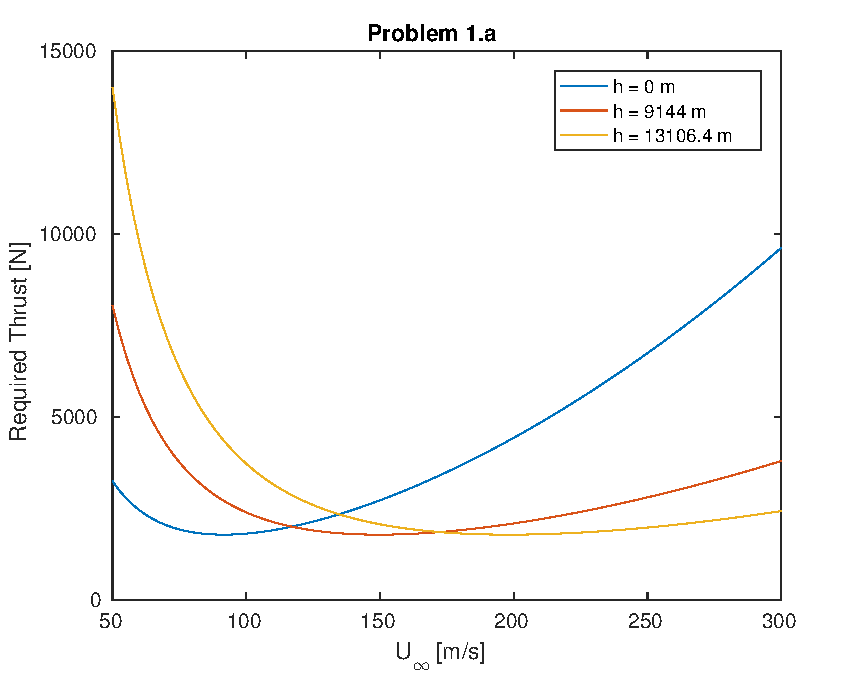
\includegraphics[width=75mm]{problem1aU.pdf}
				}
				\subfigure{
					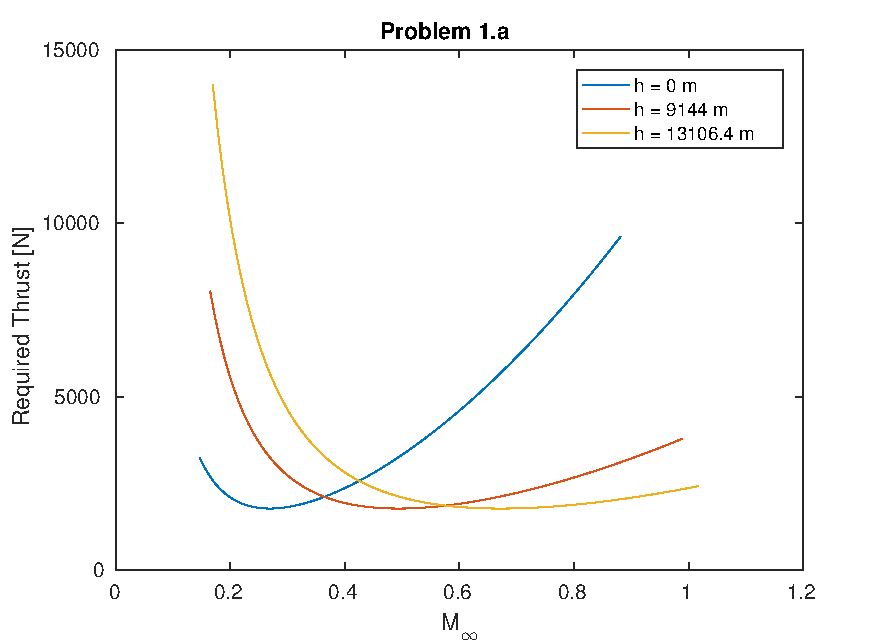
\includegraphics[width=79mm]{problem1aM.pdf}
				}
				\caption{\label{FIG_1} Plots of the required thrust against the freestream velocity and Mach number.}
			\end{center}
		\end{figure}
	\item (5 pts)
		The range, $s$, is determined from the Breguet range equation: 
		\begin{equation}
			\label{EQ_1_RANGE}
			\begin{aligned}
				\frac{W}{W_0}&=\exp\left(-\frac{s}{\mathrm{RF}}\right)\\
				\implies s&=-\mathrm{RF}\log\left(\frac{W}{W_0}\right) \\
				&=-\left(\frac{C_L}{C_D}\right)\left(\frac{U_\infty}{g\mathrm{TSFC}}\right)\log\left(\frac{W}{W_0}\right) \\
				&=-\left(\frac{C_L}{C_D}\right)\left(\frac{U_\infty}{g\mathrm{TSFC}}\right)\log\left(1-\frac{W_\mathrm{f}}{W_0}\right)\ ,
			\end{aligned}	
		\end{equation}
		where the definition of the range factor (RF) is applied between lines 2 and 3, and the relation $W=W_0-W_\mathrm{f}$ is used between lines 3 and 4.
		
		Assuming $C_L/C_D=\mathrm{const.}$, the drag is taken to be approximately 1,800 N for both altitudes, and from Eq.~\ref{EQ_1_LIFT}, $L=W_0\implies L=41,000$ N. Hence, $C_L/C_D=L/D\approx 41,000/1,800=\underline{22.7}$.
		
		Using $M_\infty=0.7$, $g\mathrm{TSFC}=0.77$ hr$^{-1}$ = $\underline{2.14\times 10^{-4}\ \mathrm{s}^{-1}}$.
		
		Since $W_\mathrm{f}=5,600$ N, $\log\left(1-W_\mathrm{f}/W_0\right)=\log\left(1-5,600/41,000\right)=\underline{-0.147}$.
		
		Upon substitution of the computed values into Eq.~\ref{EQ_1_RANGE}, $\underline{s=15,600U_\infty\ \mathrm{m}}$.
		
		For 30,000 ft., $U_{\infty,30\mathrm{kft.}}\in[140,170]\ \mathrm{m/s}\implies \boxed{s_{30\mathrm{kft.}}\in[2180,2650]\ \mathrm{km}}$. 
		
		Similarly for 43,000 ft., $U_{\infty,43\mathrm{kft.}}\in[180,230]\ \mathrm{m/s}\implies \boxed{s_{43\mathrm{kft.}}\in[2810,3590]\ \mathrm{km}}$
		
		Note that the HondaJet range is listed as 2185 km, so these values are reasonable. A few simplifications lead to a generous range calculation:
		\begin{itemize}
			\item 
				Compressibility drag is neglected.
			\item 
				$L/D=22.7$ is somewhat optimistic.
			\item 
				Some fuel is used to get to altitude, and some fuel must be kept in reserve. We have assumed all the fuel is burned during cruise, but this is an overestimate. A more realistic calculation is about $10 \%$ of fuel is used to climb and to kept in reserve: $W_\mathrm{f}=0.9\times5,600$ N $\implies s=13,900U_\infty\ \mathrm{s}$, which is about a 11\% decrease in range. (Note that for $W_\mathrm{f}/W_0\ll 1$, $s\propto W_\mathrm{f}/W_0$ by Taylor expanding the natural log function in the Breguet range equation and neglecting higher order terms).
					 
		\end{itemize}
\end{enumerate}
%%%%%%%%%%%%%%%%%%%%%%%%%%%%%%%%%%%%%%%%%%%%%%%%%%%%%%%%%%%%%%%%%%%%%%%%%%%%%%%%  
\textbf{Problem 2: The Ideal Turbojet and the Real Turbofan (60 pts)}
\begin{enumerate}[label=(\alph*)]
	\item 
		The Ideal Turbojet (20 pts)
		\begin{enumerate}[label=(\roman{*})]
			\item  (5 pts)
				Figure~\ref{FIG_2_IDEAL} shows a sketch of the ideal turbojet. For this problem it is important to show the representative geometry at each station and to show how the components are connected.
				
				\begin{figure}[!ht!]
					\begin{center}
						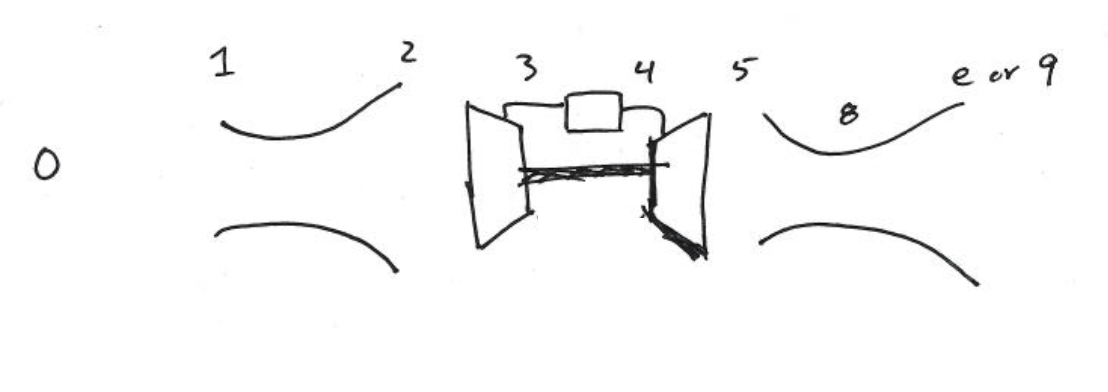
\includegraphics[width=120mm]{problem2ai.png}
						\caption{\label{FIG_2_IDEAL} Sketch of ideal turbojet with numbering conventions.}
					\end{center}
				\end{figure}
			\item (10 pts)
				Using the definition of stagnation temperature
				\begin{equation}
					\begin{aligned}
						M_e^2&=\frac{2}{\gamma-1}\left(\frac{T_{0e}}{T_e}-1\right)\ , \\
						&= \frac{2}{\gamma-1}\left(\frac{T_{05}}{T_e}\tau_n-1\right), \\
						&= \frac{2}{\gamma-1}\left(\frac{T_{05}}{T_{e}}\right)\left(\tau_n-\frac{T_{e}}{T_{05}}\right), \\
						&= \frac{2}{\gamma-1}\left(\frac{T_{05}}{T_{e}}\right)\left[\tau_n-\left(\frac{p_{e}}{p_{05}}\right)^{\frac{\gamma-1}{\gamma}}\right], \\
						\implies U_e&=\sqrt{\frac{2\gamma RT_{05}}{\gamma-1}\left[\tau_n-\left(\frac{p_{e}}{p_{05}}\right)^{\frac{\gamma-1}{\gamma}}\right]}\ .
					\end{aligned}
				\end{equation}
				Expanding this equation with the temperature and pressure ratios,
				\begin{equation}
					\label{EQ_2_UE}
					\begin{aligned}
						U_e&=\sqrt{\frac{2\gamma RT_{0}\tau_\lambda\tau_t}{\gamma-1}\left[\tau_n-\left(\frac{p_{e}}{p_{0}\pi_r\pi_d\pi_c\pi_b\pi_t}\right)^{\frac{\gamma-1}{\gamma}}\right]}\ ,
					\end{aligned}
				\end{equation}
				where $\tau_\lambda=\boxed{T_{04}/T_0}=\tau_r\tau_d\tau_c\tau_b$. For an ideal Brayton cycle, $\tau_n=\tau_d=\pi_d=\pi_b=p_e/p_0=1$. Hence,
				\begin{equation}
					\begin{aligned}
					U_e&=\boxed{\sqrt{\frac{2\gamma RT_{0}\tau_\lambda\tau_t}{\gamma-1}\left[1-\left(\pi_r\pi_c\pi_t\right)^{\frac{1-\gamma}{\gamma}}\right]}}\ , \\
					\end{aligned}
				\end{equation}
				Alternatively, in terms of just the temperature ratios and the speed of sound in the freestream state, one obtains
				\begin{equation}
				\begin{aligned}
				U_e&=a_0\sqrt{\frac{2}{\gamma-1}\left(\tau_\lambda\tau_t-\frac{\tau_\lambda}{\tau_r\tau_c}\right)}\ , \\
				\end{aligned}
				\end{equation}
				
				Now, since the work output of the turbine drives the compressor,
				\begin{equation}
					\label{EQ_2_TT}
					\begin{aligned}
						h_{04}-h_{05}&=h_{03}-h_{02}, \\
						\implies \tau_t&=1+\frac{1-\tau_c}{\tau_b\tau_c}, \\
						\tau_t&=\boxed{1+\frac{\tau_r(1-\tau_c)}{\tau_\lambda}}\ .
					\end{aligned}
				\end{equation}
				Furthermore, isentropic relations give
				\begin{equation}
					\begin{aligned}
						\tau_c&=\boxed{\pi_c^{\frac{\gamma-1}{\gamma}}}\ , \\
						\pi_t&=\boxed{\tau_t^{\frac{\gamma}{\gamma-1}}}\ , \\
						\pi_r&=\boxed{\tau_r^{\frac{\gamma}{\gamma-1}}}\ .
					\end{aligned}
				\end{equation}
				The reference temperature ratio is given by
				\begin{equation}
					\begin{aligned}
						\tau_r&=1+\frac{\gamma-1}{2}M_0^2\ , \\
							  &=\boxed{1+\frac{\gamma-1}{2\gamma RT_0}U_0^2}\ .
					\end{aligned}
				\end{equation}
				Hence, the exit velocity is now known through the above equations given $U_0$, $R$, $\gamma$, $\pi_c=p_{03}/p_{02}$, and $\tau_\lambda=T_{04}/T_{0}$.
				
				Finally, the thrust equation for an ideal Brayton cycle is given by
				\begin{equation}
					\label{EQ_2_IDEALTHRUST}					\begin{aligned}
						T&=\dot m_A (U_e-U_0)+A_e(p_e-p_0)\ , \\
						&= \boxed{\dot m_A (U_e-U_0)}\ .
					\end{aligned}
				\end{equation}
			\item (5 pts)
				$U_0=0$ since the static thrust is desired. Hence,  $\tau_r=1\implies \pi_r=1$ and from Eq.~\ref{EQ_2_IDEALTHRUST}, $T=\dot m_A U_e$.
				
				Furthermore, $\tau_\lambda=T_{04}/T_0=1600/288.15=5.55$, and $\tau_c=24^{(1.4-1)/1.4}=2.48$. Using Eq.~\ref{EQ_2_TT}, $\tau_t=0.734\implies \pi_t=0.338$.
				
				Finally by substituting the computed values into Eq.~\ref{EQ_2_UE}, one obtains $U_e=1,030$ m/s $\implies \boxed{T=8,240}$ N.
				
				The Honda HF-120 lists the take-off thrust at 2,095 lbf $\approx$ 9,300 N. A few differences are
				\begin{itemize}
					\item
						Our model is a turbojet, HF-120 is a turbofan
					\item	 
						Engines are typically tested in isolated fixtures but when installed on an aircraft, actual thrust is slightly lower (nacelles, etc.) 	
				\end{itemize} 
				Note that we still underpredict the thrust even in an ideal configuration.
		\end{enumerate}
%%%%%%%%%%%%%%%%%%%%%%%%%%%%%%%%%%%%%%%%%%%%%%%%%%%%%%%%%%%%%%%%%%%%%%%%%%%%%%%%
	\item (25 pts)
		The Real Turbofan
		\begin{enumerate}[label=(\roman{*})]
			\item  (5 pts)
			Figure~\ref{FIG_2_REAL} shows a sketch of the real turbofan. For this problem, one should ensure that the correct connectivities are shown.
			
			\begin{figure}[!ht!]
				\begin{center}
					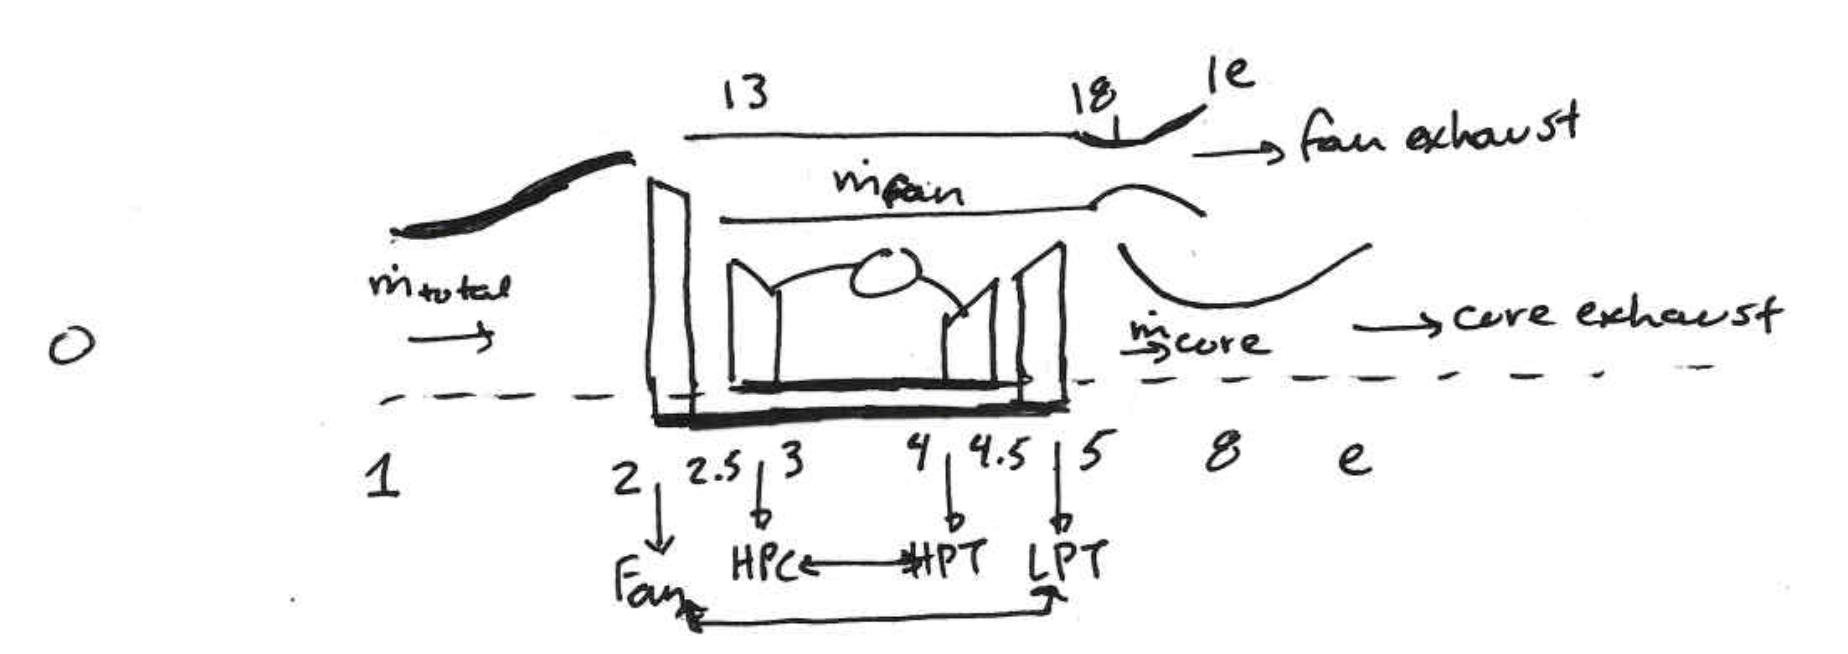
\includegraphics[width=120mm]{problem2bi.png}
					\caption{\label{FIG_2_REAL} Sketch of the real turbofan.}
				\end{center}
			\end{figure}
		
			\item (15 pts)
				The thrust for a turbofan is given by 
				\begin{equation}
					\label{EQ_2_TFTHRUST}					\begin{aligned}
						T&=\boxed{\dot m_c [(U_e-U_0)+\beta(U_{1e}-U_0)]}\ .
					\end{aligned}
				\end{equation}
				where the exit pressure is assumed to be the same as the initial state and the injection of fuel is not considered. Additionally, the bypass ratio is given by $\beta=\dot m_f /\dot m_c$.
				
				Enthalpy conservation for an adiabatic nozzle gives
				\begin{equation}					
					\begin{aligned}
						h_e+\frac{1}{2}U_e^2&=h_{05}\ , \\ 
						\implies U_e&=\sqrt{2(h_{05}-h_e)}\ , \\
						&=\sqrt{2\eta_N(h_{05}-h_{es})}\ , \\
						&=\sqrt{2\eta_Nc_p(T_{05}-T_{es})}\ , \\
						&=\sqrt{2\eta_Nc_pT_{05}\left(1-\frac{T_{es}}{T_{05}}\right)}\ , \\
						&=a_0\sqrt{\frac{2\eta_N\tau_\lambda\tau_t}{\gamma-1}\left(1-\frac{T_{es}}{T_{05}}\right)}\ . \\
					\end{aligned}
				\end{equation}
				Since $T_{es}/T_{05}$ is an isentropic process, we may rewrite the above as
				\begin{equation}					
					\begin{aligned}
						U_e&=a_0\sqrt{\frac{2\eta_N\tau_\lambda\tau_{hpt}\tau_{lpt}}{\gamma-1}\left[1-\left(\frac{p_{es}}{p_{05}}\right)^{\frac{\gamma-1}{\gamma}}\right]}\ , \\
						&=a_0\sqrt{\frac{2\eta_N\tau_\lambda\tau_{hpt}\tau_{lpt}}{\gamma-1}\left[1-\left(\frac{p_{es}}{p_0\pi_r\pi_d\pi_f\pi_c\pi_b\pi_{t}}\right)^{\frac{\gamma-1}{\gamma}}\right]}\ , \\ \\
						&=\boxed{a_0\sqrt{\frac{2\eta_N\tau_\lambda\tau_t}{\gamma-1}\left[1-\left(\pi_r\pi_d\pi_f\pi_c\pi_{t}\right)^{\frac{1-\gamma}{\gamma}}\right]}}\ . \\
					\end{aligned}
				\end{equation}
				where it is assumed that $p_{es}=p_0$ and $\pi_b=1$ since $\eta_b=1$. Also, $\tau_{hpt}\tau_{lpt}=\tau_t$.
				
				Similarly, the exit velocity from the fan is found to be
				
				\begin{equation}					
					\begin{aligned}
						U_{e1}&=\boxed{a_0\sqrt{\frac{2\eta_{N1}\tau_r\tau_d\tau_f}{\gamma-1}\left[1-\left(\pi_r\pi_d\pi_f \right)^{\frac{1-\gamma}{\gamma}}\right]}}\ .  
					\end{aligned}
				\end{equation}
				
				The matching conditions between the high-pressure turbine and the compressor are similar to before:
				
				\begin{equation}
					\begin{aligned}
						h_{04}-h_{04.5}&=h_{03}-h_{02.5}, \\
						\implies \tau_{hpt}&=1+\frac{1-\tau_c}{\tau_b\tau_c}, \\
						\tau_{hpt}&=\boxed{1+\frac{\tau_r\tau_d\tau_f(1-\tau_c)}{\tau_\lambda}}
					\end{aligned}
				\end{equation}
				
				For the matching conditions between the low-pressure turbine and the fan, the two separate streams in the fan must be accounted for: 
				
				\begin{equation}
					\begin{aligned}
						\dot{m}_c(h_{04.5}-h_{05})&=\dot{m}_c h_{02.5}+\dot{m}_f h_{013}-(\dot{m}_c+\dot{m}_f)h_{02}\ , \\
						\implies T_{04.5}-T_{05}&=T_{02.5}+\beta T_{013}-(1+\beta)T_{02}\ .
					\end{aligned}
				\end{equation}
				
				Assuming $T_{02.5}=T_{013}$,
				 \begin{equation}
					 \begin{aligned}
						 T_{04.5}-T_{05}&=(1+\beta)(T_{02.5}-T_{02})\ , \\
						 \implies \tau_{lpt}&=1+\frac{(1+\beta)(1-\tau_f)}{\tau_{hpt}\tau_b\tau_c\tau_f}, \\
						 \tau_{lpt}&=\boxed{1+\frac{\tau_r\tau_d(1-\tau_f)(1+\beta)}{\tau_\lambda\tau_{hpt}}}
					 \end{aligned}
				 \end{equation}
				 
				 For the diffuser, the adiabatic efficiency yields the temperature ratio
				 
				 \begin{equation}
					 \begin{aligned}
						 \eta_d &= \frac{h_{02s}-h_{0}}{h_{02}-h_{0}}\ , \\ 
						 & = \frac{T_{02s}/T_{0}-1}{T_{02}/T_{0}-1} , \\
						 & = \frac{\left(\pi_d\pi_r\right)^{\frac{\gamma-1}{\gamma}}-1}{\tau_d\tau_r-1} \\ ,
						 & = \frac{\left(\pi_d\pi_r\right)^{\frac{\gamma-1}{\gamma}}-1}{\tau_r-1} \\ ,
						 \implies \pi_d&=\boxed{\frac{\left[1+\eta_d\left(\tau_r-1\right)\right]^{\frac{\gamma}{\gamma-1}}}{\pi_r}}
					 \end{aligned}
				 \end{equation}
				 where the fourth line follows the third by the assumption that $\boxed{\tau_d\approx 1}$. 
				 
				 Similarly, the adiabatic efficiencies for the compressor, fan, and turbine give 
				 
				 \begin{equation}
					 \begin{aligned}
						 \tau_c &=\boxed{1+\frac{1}{\eta_c}\left(\pi_c^{\frac{\gamma-1}{\gamma}}-1\right)}\ , \\
						 \tau_f &=\boxed{1+\frac{1}{\eta_f}\left(\pi_f^{\frac{\gamma-1}{\gamma}}-1\right)}\ , \\
						 \pi_t &=\boxed{\left[1+\eta_t(\tau_t-1) \right]^{\frac{\gamma}{\gamma-1}}}\ .
					 \end{aligned}
				 \end{equation}
			\item (5 pts)
			
			Using the equations given above, the sea level static thrust is found to be \boxed{14.4\ \mathrm{kN}}. The Honda Jet produces a thrust of 2095 lbf = 9.32 kN. Hence, the model predicts the sea level thrust to be much higher than actual.
			
		\end{enumerate}
%%%%%%%%%%%%%%%%%%%%%%%%%%%%%%%%%%%%%%%%%%%%%%%%%%%%%%%%%%%%%%%%%%%%%%%%%%%%%%%%
	\item (15 pts)
	Comparison of the Ideal Turbojet and the Real Turbofan
	\begin{enumerate}[label=(\roman{*})]
		\item (10 pts)
			Plots of the real turbofan and the ideal turbojet thrust are shown in Fig.~\ref{FIG_3_COMPARE}. Note that the thrust is the total thrust from the two engines attached to the Honda Jet.
			
			\begin{figure}[!ht!]
				\begin{center}
					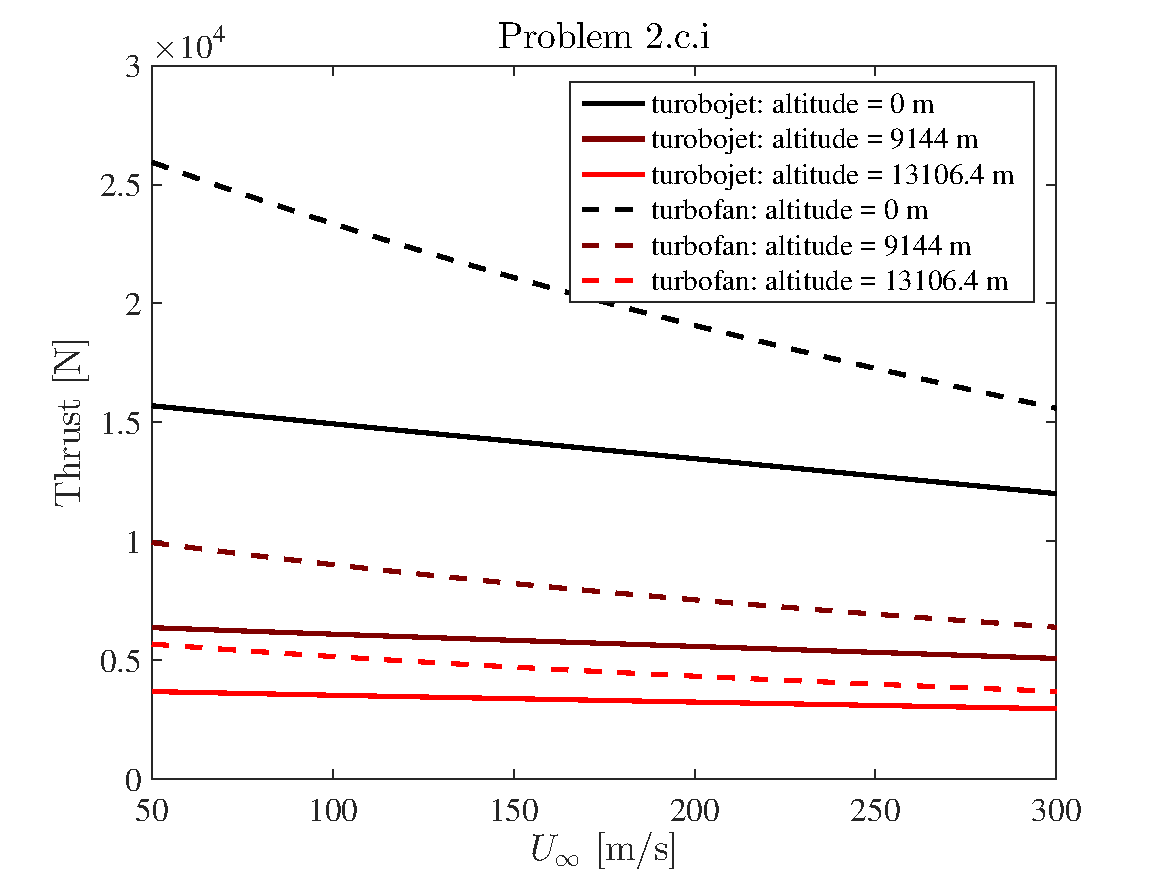
\includegraphics[width=120mm]{problem2ci.pdf}
					\caption{\label{FIG_3_COMPARE} Comparison of the computed real turbofan thrust with the ideal turbojet. Note that the thrust produced by both engines is shown.}
				\end{center}
			\end{figure}
		\item (5 pts)
			We see that at low speeds turbofans are much better. However, thrust drops more sharply as speed increases for the turbofan; this indicates that turbofans may not be as advantageous at high speeds. Hence, military aircraft tend to use low bypass ratio turbofans since they operate at higher speeds.
			
			
			For very large bypass ratios, practical considerations with respect to the size of the engine come into play; that is, the engine may not fit on the airframe and the weight may be too high (i.e., the engine starts to adversely affect the $L/D$ ratio). 
			
			High bypass ratio engines are around 9-10 today. Note that the Pratt and Whitney PW1000G family of engines are \textbf{geared} turbofans with bypass ratios up to 12. 
	\end{enumerate}
		
\end{enumerate}
%%%%%%%%%%%%%%%%%%%%%%%%%%%%%%%%%%%%%%%%%%%%%%%%%%%%%%%%%%%%%%%%%%%%%%%%%%%%%%%%
\end{document}